\documentclass[a4paper,12pt,twoside]{scrreprt}
% Autor der Vorlage: Klaus Rheinberger, FH Vorarlberg
% 2017-02-20

%% Hilfe: z.B.
% empfohlener Einstieg: http://latex.tugraz.at/  
% https://de.wikibooks.org/wiki/LaTeX-Kompendium:_Schnellkurs:_Erste_Schritte
% https://de.wikibooks.org/wiki/LaTeX-Kompendium:_Schnellkurs
% https://de.wikibooks.org/wiki/LaTeX-Kompendium

%% Pakete:
% Der Befehl \usepackage[latin9]{inputenc} ermöglicht die direkte Angabe von Umlauten. Übrigens lässt sich so auch das Euro-Zeichen direkt eingeben. Auf Betriebssystemen, wie zum Beispiel allen neueren Linux-Distributionen, verwendet man statt \usepackage[latin9]{inputenc} besser \usepackage[utf8]{inputenc}, auf Applesystemen verwendet man \usepackage[macce]{inputenc} (oder das für ältere Modelle gültige \usepackage[applemac]{inputenc}).
\usepackage[utf8]{inputenc}
\usepackage[T1]{fontenc}    % Silbentrennung bei Sonderzeichen
\usepackage{graphicx}       % Bilder einbinden
\usepackage[ngerman]{babel} % Deutsche Sprachanpassungen
\usepackage{csquotes}       % When using babel or polyglossia with biblatex, loading csquotes is recommended to ensure that quoted texts are typeset according to the rules of your main language.
\usepackage{acronym}  % für optionales Abkürzungsverzeichnis
\usepackage{eurosym}  % z. B. \EUR{12345,68}
\usepackage[linktocpage=true]{hyperref} % Links z. B. \href{https://www.wikibooks.org}{Wikibooks home}
\usepackage[bindingoffset=8mm]{geometry}% Bindeverlust von 8mm einbeziehen. Mit dem geometry-Paket können Sie die Ränder auch ganz individuell anpassen.
\usepackage{caption} % Abbildungslegenden
\captionsetup{format=hang, justification=raggedright}

\usepackage[style=ieee,citestyle=ieee,backend=biber]{biblatex}   % Literaturverweise
%\usepackage[style=numeric,citestyle=numeric,backend=biber]{biblatex}
% biblatex comes with a variety of built-in bibliography/citation style families (numeric, alphabetic, authoryear, authortitle, verbose), and there's a growing number of custom styles:
% https://de.sharelatex.com/learn/Biblatex_citation_styles
% https://de.sharelatex.com/learn/Biblatex_bibliography_styles
\addbibresource{Zotero-Beispiele.bib}    % Zotero-Beispiele.bib ist die verwendete Bibtex-Datei 
% Anstatt die Bibtex-Datei selber zu erstellen, kann sie z. B. aus einer Zotero-Sammlung zu BibTeX exportiert werden.


%% Einstellungen:
\setcounter{secnumdepth}{4}
\setcounter{tocdepth}{4}   % Tiefe der Gliederung im In haltsverzeichnis


%% ERSETZEN VON ECKIGEN KLAMMERN:
% Ersetzen Sie den Text in den eckigen Klammern!

\begin{document}

% evtl. Sperrvermerkseite
\thispagestyle{empty}

\noindent
[Achtung: Verwenden Sie einen Sperrvermerk nur in sehr gut begründeten Fällen!] 

\section*{[evtl. Sperrvermerk]}   % evtl. ersetzen durch \section*{Sperrvermerk}
Die vorliegende Arbeit ist bis zum [DATUM] für die öffentliche Nutzung zu sperren. Veröffentlichung, Vervielfältigung und Einsichtnahme sind ohne meine ausdrückliche Genehmigung nicht gestattet. Der Titel der Arbeit sowie das Kurzreferat/Abstract dürfen veröffentlicht werden.

\vspace{3cm}

\noindent Dornbirn, \hfill Unterschrift Verfasser*in


% Titelblatt:
% \newpage\mbox{}\newpage
\cleardoublepage   % force output to a right page
\thispagestyle{empty}
\begin{titlepage}
  \begin{flushright}
  
\includegraphics[width=0.4\linewidth]{Logo-A3}
  \end{flushright}
  \begin{flushleft}
  \section*{[Titel der Arbeit]}
  \subsection*{[Untertitel der Arbeit]}
  \vspace{1cm}
  
  [Master/Bachelor]arbeit\\
  zur Erlangung des akademischen Grades
  \vspace{0.5cm}
  
  \textbf{[z. B. Master of Science in Engineering (MSc)]}

  \vspace{1cm}
  Fachhochschule Vorarlberg\newline
  [z. B. Nachhaltige Energiesysteme]

  \vspace{0.5cm}
  
  Betreut von\newline
  [Name(n) der betreuenden Lehrperson(en)]
  
  \vspace{0.5cm}
  
  Vorgelegt von\newline
  [Name(n) Verfasser*in(nen)]\newline
  Dornbirn, [Monat Jahr]
  \end{flushleft}
\end{titlepage}


% evtl. Widmung:
\newpage
\section*{[evtl. Widmung]}   % evtl. ersetzen durch \section*{Widmung}

[Text der Widmung]

% Kurzreferat:
\newpage
\section*{Kurzreferat}

\subsection*{[Deutscher Titel Ihrer Arbeit]}

[Text des Kurzreferats]
\vspace{0.5cm}

\noindent
[Evtl. 5-7 Schlagwörter:]

% Abstract:
\newpage
\section*{Abstract}
\subsection*{[English Title of your thesis]}

[text of the abstract]
\vspace{0.5cm}

\noindent
[Optionally 5-7 keywords:]

% evtl. Vorwort:
\newpage
\section*{[evtl. Vorwort]}   % evtl. ersetzen durch \section*{Widmung}

[Text des Vorworts]


% Inhaltsverzeichnis:
\cleardoublepage   % force output to a right page
\tableofcontents

\clearpage
\phantomsection
\addcontentsline{toc}{chapter}{Abbildungsverzeichnis}
\listoffigures

\clearpage
\phantomsection
\addcontentsline{toc}{chapter}{Tabellenverzeichnis}
\listoftables

% evtl. Abkürzungsverzeichnis:
\clearpage
\phantomsection
\addcontentsline{toc}{chapter}{[evtl. Abkürzungsverzeichnis]}  % evtl. ersetzen durch \addcontentsline{toc}{chapter}{Abkürzungsverzeichnis}
\chapter*{[evtl. Abkürzungsverzeichnis]} % evtl. ersetzen durch \chapter*{Abkürzungsverzeichnis}
\begin{acronym}[SQL]
 \acro{ETW}{Energietechnik und Energiewirtschaft}
 \acro{SQL}{Structured Query Language}
 \acro{Bash}{Bourne-again shell}
\end{acronym}

%% Die Kapitelstruktur ist mit der betreuungsperson abzustimmen!

\chapter{[Kapitel]}
Formatvorlage für den Fließtext. Formatvorlage für den Fließtext. Formatvorlage für den Fließtext. Formatvorlage für den Fließtext. Formatvorlage für den Fließtext. Formatvorlage für den Fließtext. Formatvorlage für den Fließtext. Formatvorlage für den Fließtext. Formatvorlage für den Fließtext. Formatvorlage für den Fließtext. Formatvorlage für den Fließtext.
\begin{quote}
  Formatvorlage für ein längeres direktes Zitat. Formatvorlage für ein längeres direktes Zitat. Formatvorlage für ein längeres direktes Zitat. Formatvorlage für ein längeres direktes Zitat. Formatvorlage für ein längeres direktes Zitat. Formatvorlage für ein längeres direktes Zitat….
\end{quote}

\EUR{12345,68}, \href{https://www.wikibooks.org}{Wikibooks home}

\chapter{[Kapitel]}
Formatvorlage für den Fließtext.
Hier eine Liste.
\begin{enumerate}
 \item Verstehen
 \item Üben
 \item Können
\end{enumerate}


\section{[Unterkapitel zweite Ebene]}
Formatvorlage für den Fließtext. Die Abbildung~\ref{fig:ex} auf Seite \pageref{fig:ex} zeigt drei Entladungskurven eines biphasischen Defibrillators.
\begin{figure}[htb]
  \centering
  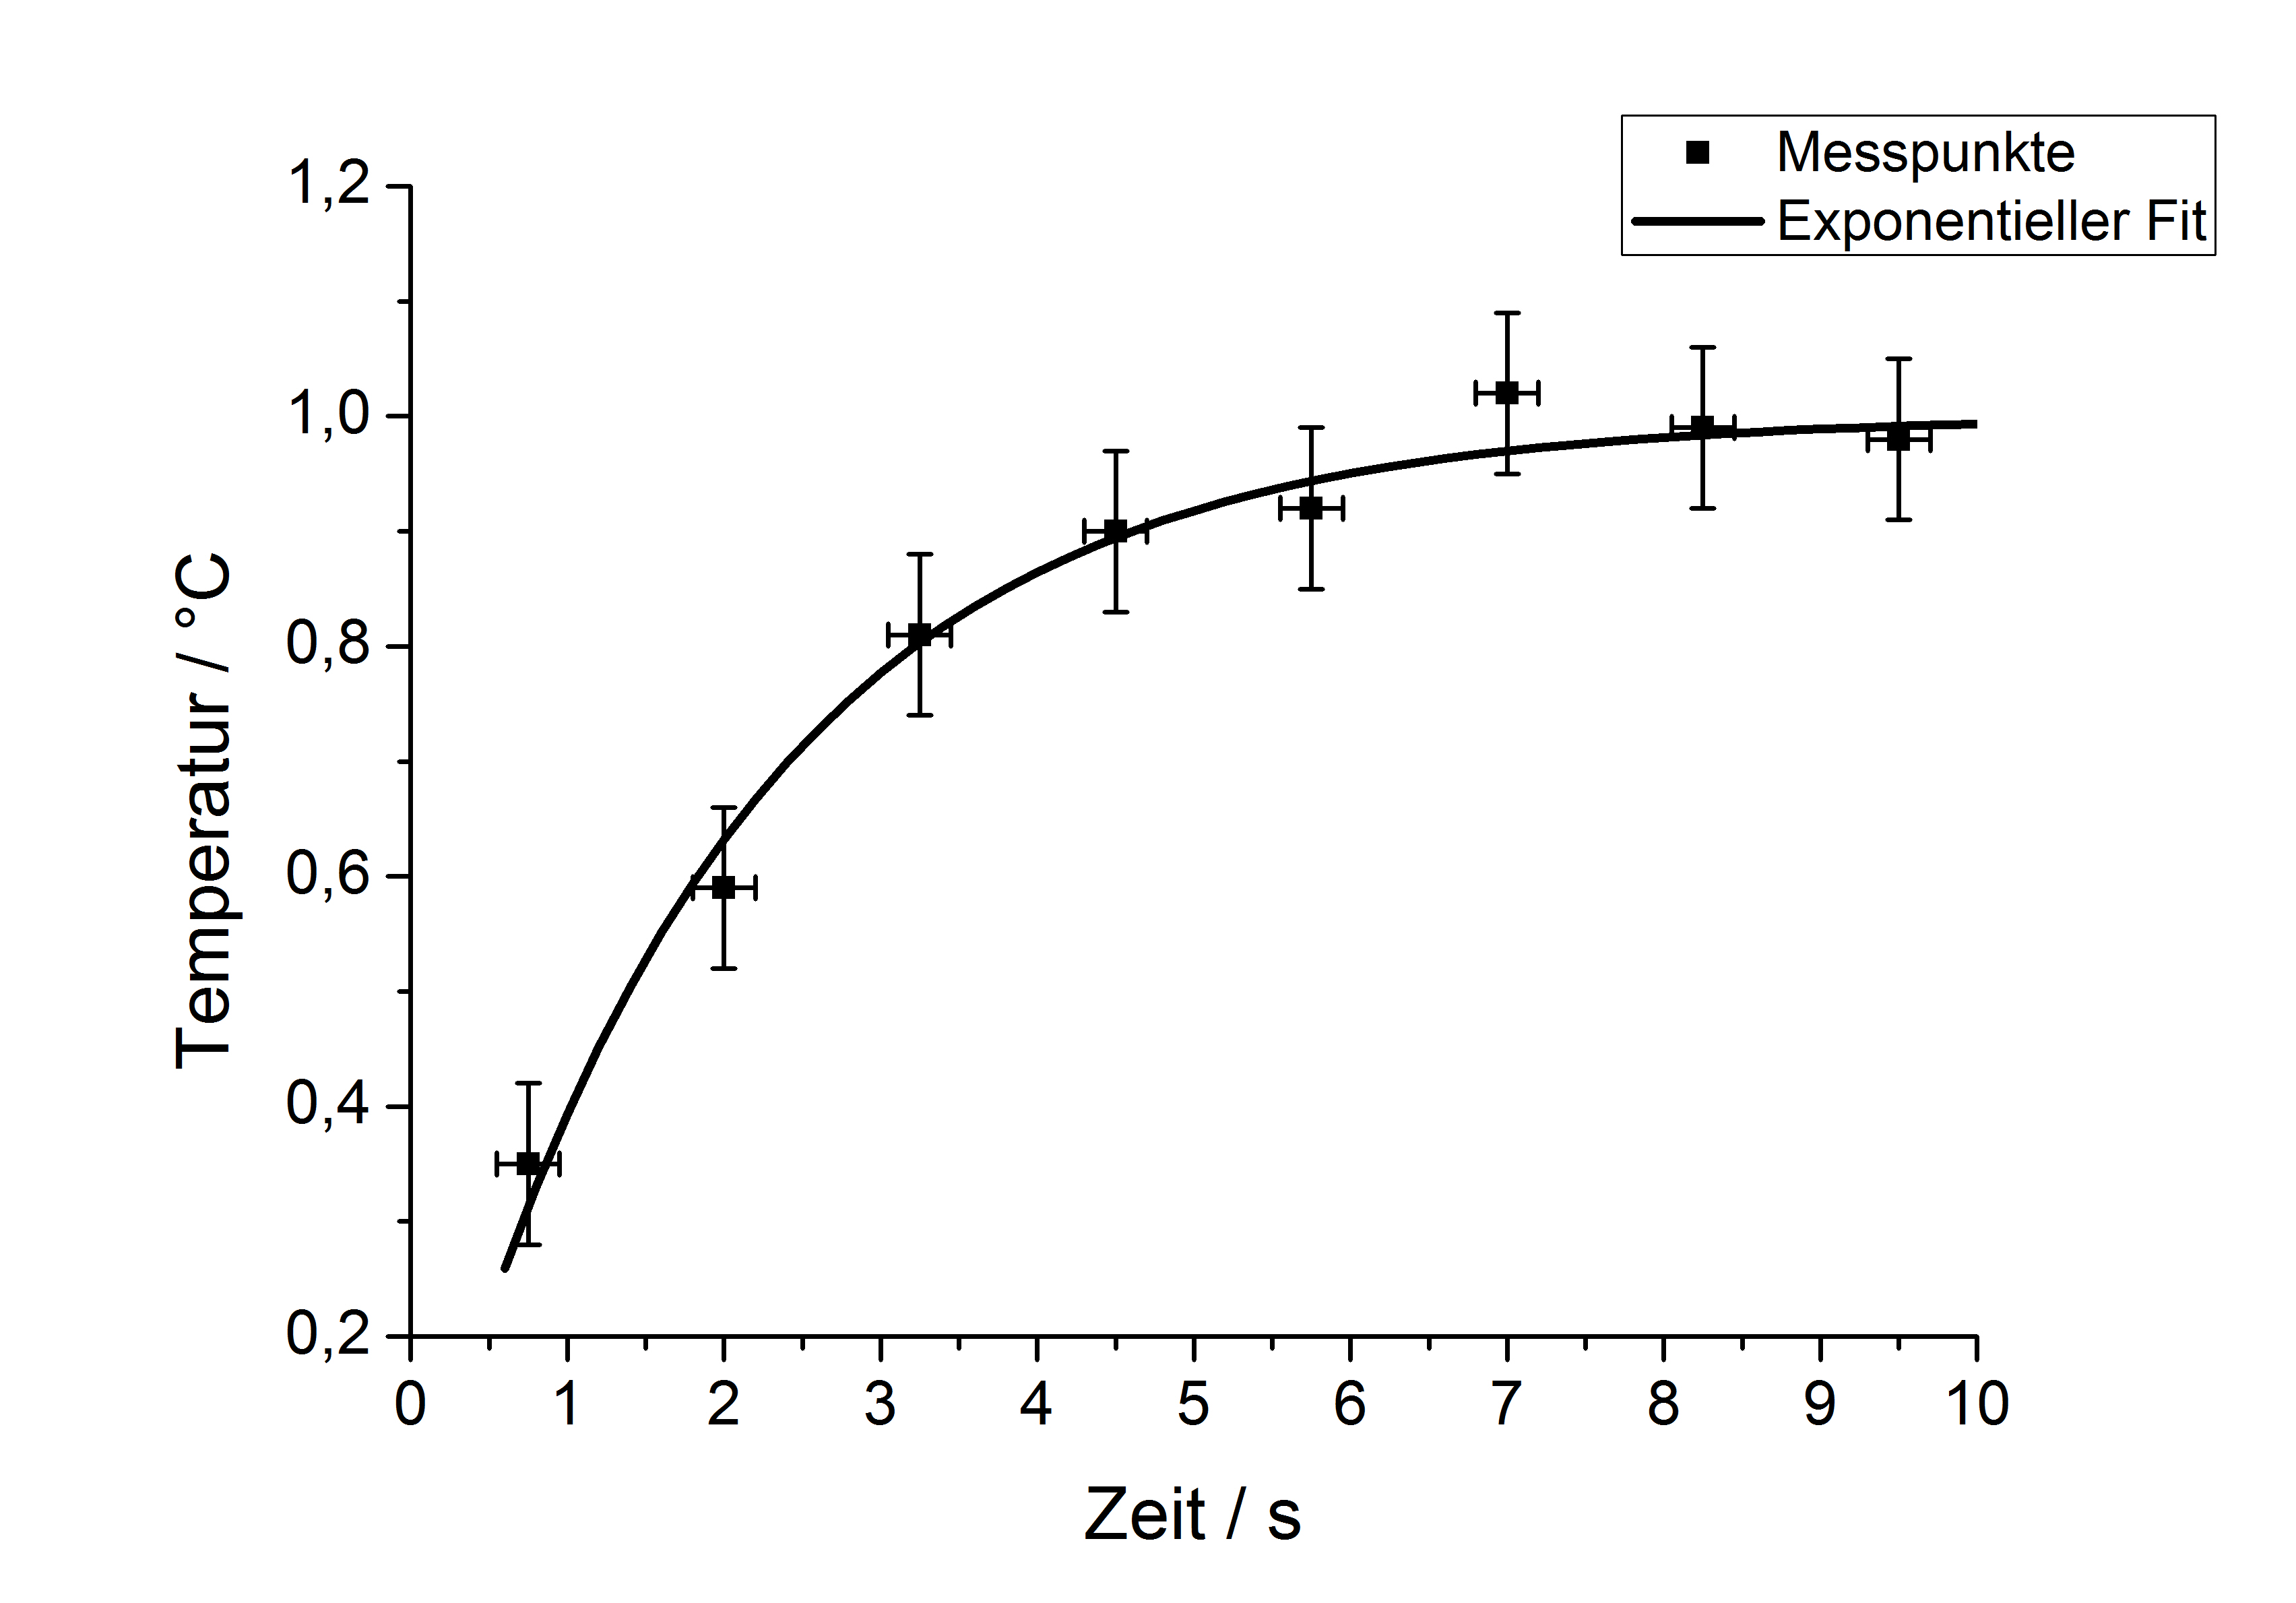
\includegraphics[width=10cm]{Amann_TechnAbb}
  \caption[Aufheizverhalten von PTFE]{Aufheizverhalten von PTFE. \\Quelle: eigene Ausarbeitung}
 \label{fig:ex}
\end{figure}


\section{[Unterkapitel zweite Ebene]}
Formatvorlage für den Fließtext.
Jetzt eine Fußnote\footnote{Dies ist eine Fußnote.}
Die quadratischen Gleichung (\ref{equ:foo}) hat wieviele Nullstellen?
\begin{equation}
 \label{equ:foo}
 x^2-2x+5=0.
\end{equation}
Zwei von Einsteins berühmtesten Formeln lauten:
\begin{eqnarray*}
  E &= mc^2                                  \\
  m &= \frac{m_0}{\sqrt{1-\frac{v^2}{c^2}}}
\end{eqnarray*}


\subsection{[Unterkapitel dritte Ebene]}
Formatvorlage für den Fließtext. Hier die einfache Tabelle \ref{tab:sp}

\begin{table}[htb]
  \centering
  \begin{tabular}{ | l | l |c|}
    \hline
    Datum      & Thema           & Raum \\
    \hline\hline
    Montag     & Graphentheorie  & U1   \\
    \hline
    Donnerstag & Algebra         & MZB23\\
    \hline
  \end{tabular}
  \caption[Stundenplan]{Stundenplan des Jahres 2030.\\Quelle: eigene Ausarbeitung}
  \label{tab:sp}
\end{table}

\subsubsection{[Unterkapitel vierte Ebene]}
Formatvorlage für den Fließtext.



\section{[Unterkapitel zweite Ebene]}

Verweise: zu einem Buch mit Details \cite[vgl.][Kapitel 2]{bathe_finite-elemente-methoden_1990} oder ohne Details \cite{bathe_finite-elemente-methoden_1990}, ein Buchteil \cite{areger_problem-based_2007}, eine Dissertation \cite{sporn_interaktives_2000}, ein Dokument \cite{industriellenvereinigung_beste_2014}, ein Enzyklopädieartikel \cite{brockhaus_kreativitat_1872}, ein Film \cite{de_wilde_through_2008}, ein Konferenz-Paper \cite{weber_podcasts._2006}, ein Magazin-Artikel \cite{autornachname1_magazinartikeltitel_1995}, ein Pordcast \cite{paulus_horen_????}, eine Tonaufnahme \cite{horowitz_horowitz_2003}, eine Videoaufnahme \cite{fhvlearningsupport_was_2008}, ein Vortrag \cite{kohls_literaturverwaltung_2008}, eine Website \cite{wedekind_von_2008}, ein Zeitschriftenartikel \cite{hofer_wir_2008} und ein Zeitungsartikel \cite{schenkel_tsunami_2012}.


\chapter{[Kapitel]}

\section{[Unterkapitel zweite Ebene]}
Formatvorlage für den Fließtext.

\subsection{[Unterkapitel dritte Ebene]}
Formatvorlage für den Fließtext.

\subsubsection{[Unterkapitel vierte Ebene]}
Formatvorlage für den Fließtext.


% Literaturverzeichnis:
\clearpage
\phantomsection
\addcontentsline{toc}{chapter}{Literaturverzeichnis}
\printbibliography


\chapter*{[evtl. Anhang]}  % evtl. ersetzen mit \chapter*{Anhang}
\addcontentsline{toc}{chapter}{[evtl. Anhang]}   % evtl. ersetzen mit \addcontentsline{toc}{chapter}{Anhang}
Formatvorlage für den Fließtext.


\chapter*{Eidesstattliche Erklärung}
\addcontentsline{toc}{chapter}{Eidesstattliche Erklärung}
Ich erkläre hiermit an Eides statt, dass ich die vorliegende [Master - bzw. Bachelor]arbeit selbstständig und ohne Benutzung anderer als der angegebenen Hilfsmittel angefertigt habe. Die aus fremden Quellen direkt oder indirekt übernommenen Stellen sind als solche kenntlich gemacht. Die Arbeit wurde bisher weder in gleicher noch in ähnlicher Form einer anderen Prüfungsbehörde vorgelegt und auch noch nicht veröffentlicht.

\vspace{3cm}
\noindent
Dornbirn, am [Tag. Monat Jahr anführen]\hfill [Vor- und Nachname Verfasser*in]


\end{document}
